\chapter{Background}

\section{Convolutional Encoding}

Convolutional Codes are a type of error correcting code (ECC) that use memory storing elements and convolution of a message with a generator polynomial to encode each transmitted bit. In this chapter we use the notion described in \Table~\tref{Table:Background:SymbolDefinitions}.

%%%%%%%%%%%%%%%%%%%%%%%%%%%%%%%%%%%%%%%%%%%%%%%%%%%%%%%%%%%%%%%%%
% TABLE: BACKGROUND: Symbol Definitions
\begin{table}
\caption[Background chapter symbols and definitions]
{Background chapter symbols and definitions}
\label{Table:Background:SymbolDefinitions}
\centering\CaptionFontSize
\begin{tabular}{c@{\hspace{1em}}l}
\toprule
Symbol & Definition
\\
\midrule
$N$ & number of memory storing elements (number of bits in a state)
\\
$T$ & length of pre-encoded message in bits
\\
$k$ & rate of the encoder (1/k); we use a rate 1/5 (k=5) encoder in our simulations
\\

\bottomrule
\end{tabular}
\end{table}
%%%%%%%%%%%%%%%%%%%%%%%%%%%%%%%%%%%%%%%%%%%%%%%%%%%%%%%%%%%%%%%%%

\subsection{Generator Polynomial and Convolution}

At a basic level, Convolutional Codes encode a message by performing a discrete time convolution on a stream of message bits. This is done by storing the N previous bits streamed and then performing a series of XORs operations with them and the next bit to result in an encoding. The series of XORs (1-bit XOR is equivalent to addition) performed defines the generator polynomial that we are convolving with the pre-encoded message. An example of this is shown in \Figure~\fref{Figure:Background:ConvolutionalEncoderArchitecture}. 

%%%%%%%%%%%%%%%%%%%%%%%%%%%%%%%%%%%%%%%%%%%%%%%%%%%%%%%%%%%%%%%%%
% FIGURE: BACKGROUND: Convolutional Encoder Architecture
\begin{figure}
\centering\CaptionFontSize
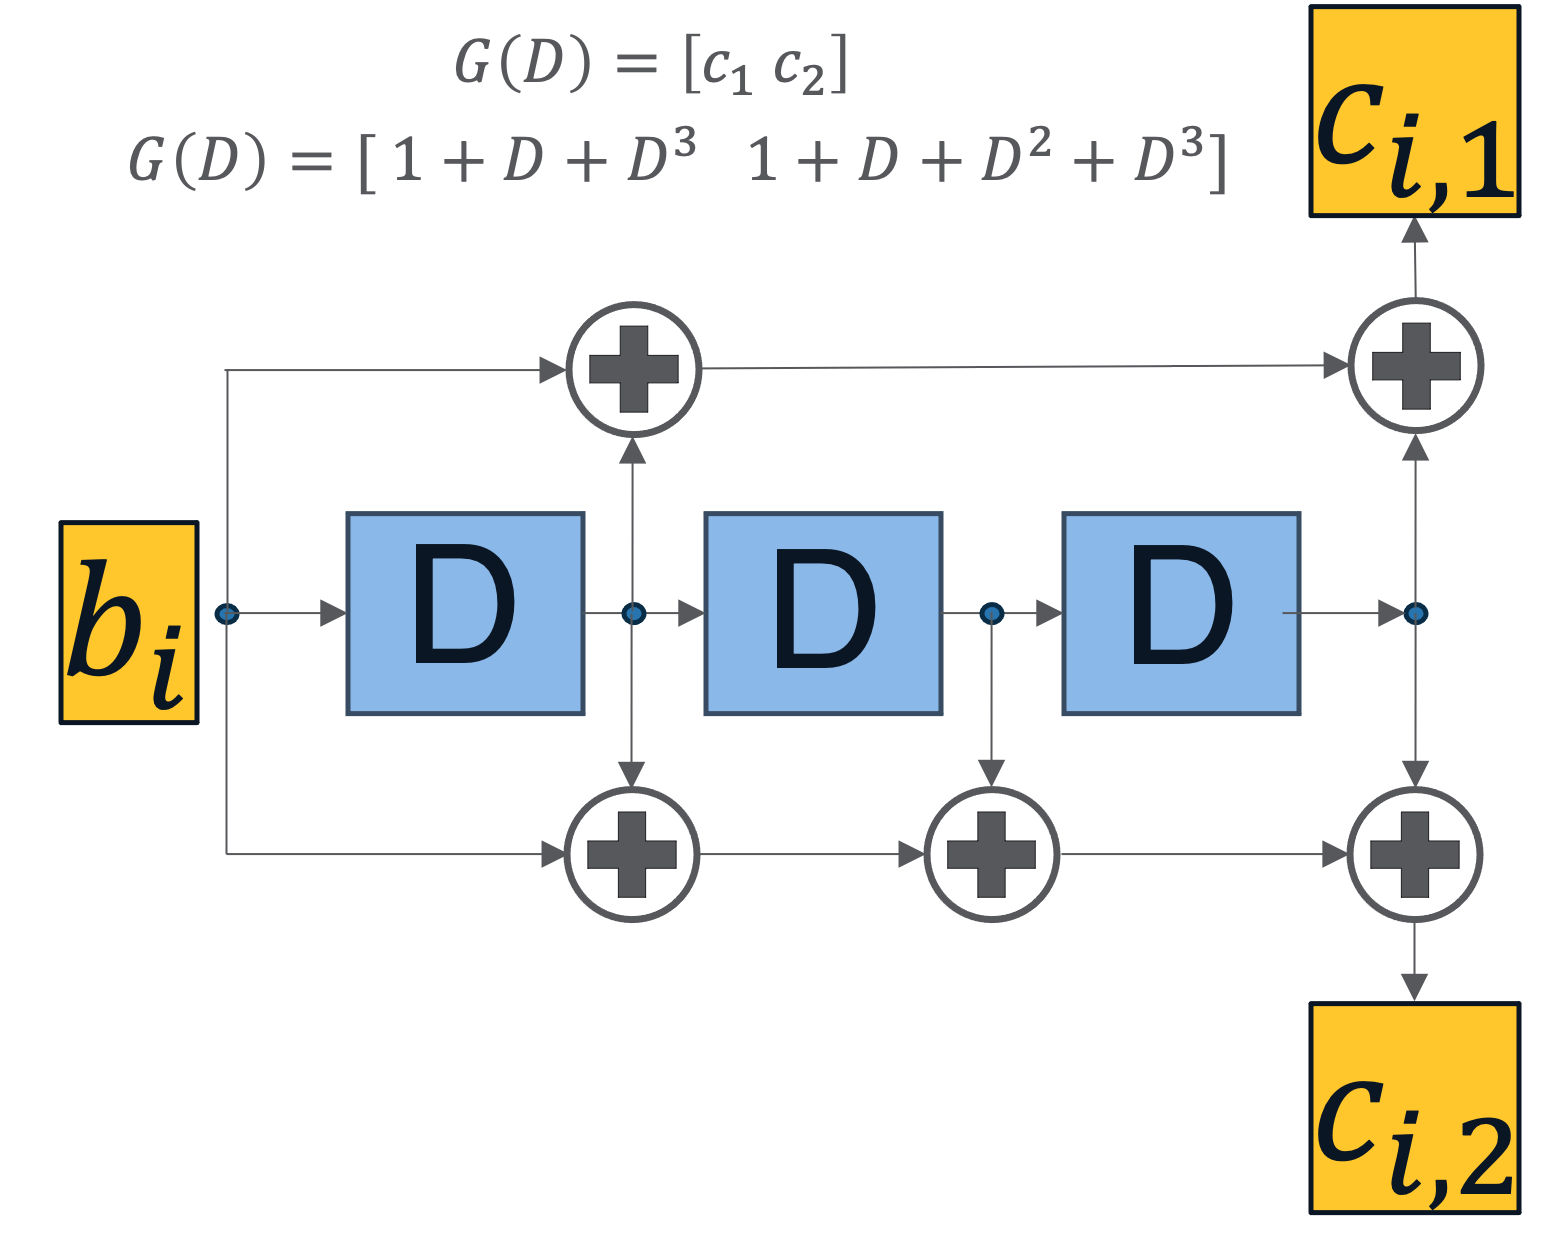
\includegraphics[height=15em]
{Figures/convolutional_encoding_hw.png}
\caption[Implementation of a convolutional encoder with a given generator polynomial]
{Implementation of a convolutional encoder with a given generator polynomial}
\label{Figure:Background:ConvolutionalEncoderArchitecture}
\end{figure}
%%%%%%%%%%%%%%%%%%%%%%%%%%%%%%%%%%%%%%%%%%%%%%%%%%%%%%%%%%%%%%%%%

Here $(u_n)$ is the sequence of bits being streamed and $c_{1,i}$ and $c_{2,i}$ correspond to the (in this example) two bit encoding of $u_i$. Furthermore, each memory storing element $D$ is cascaded and will store and output the last value that was at its input. Thus, based on the above architecture, each $u_i$ is encoded to $[c_{1,i} \quad c_{2,i}]$ where 
$$[c_{1,i} \quad c_{2,i}] = [ u_i + u_{i-1} + u_{i-3} \quad u_i + u_{i+1} + u_{i+2} + u_i]$$

In other words, the sequence $c = [(c_1,n)  \quad (c_2,n) ]$ is a discrete convolution of $(u_n)$ with the sequence $(g_n) =  [ [1  1 0 1] \quad [1 1 1 1]]$. In the polynomial representation, $c(D) = u(D)G(D)$, the generator polynomial that then represents this specific encoding would be 
$$G(D) =	[1 + D + D^3  \quad 1+ D + D^2 + D^3]$$

It is worth noting that the output of the encoder will output the sequence $c$ in the following format
$$c = (c_{1,0}, c_{2,0}, c_{1,1}, c_{2,1}, \ldots, c_{1,i}, c_{2,i}, \ldots, c_{1,T}, c_{2,T})$$

\subsection{State Diagram Representation}
A useful interpretation of the encoding process is as transitions in a state diagram as shown in \Figure~\fref{Figure:Background:ConvolutionalCodeStateDiagram}.

%%%%%%%%%%%%%%%%%%%%%%%%%%%%%%%%%%%%%%%%%%%%%%%%%%%%%%%%%%%%%%%%%
% FIGURE: BACKGROUND: Convolutional Encoder State Diagram
\begin{figure}
\centering\CaptionFontSize
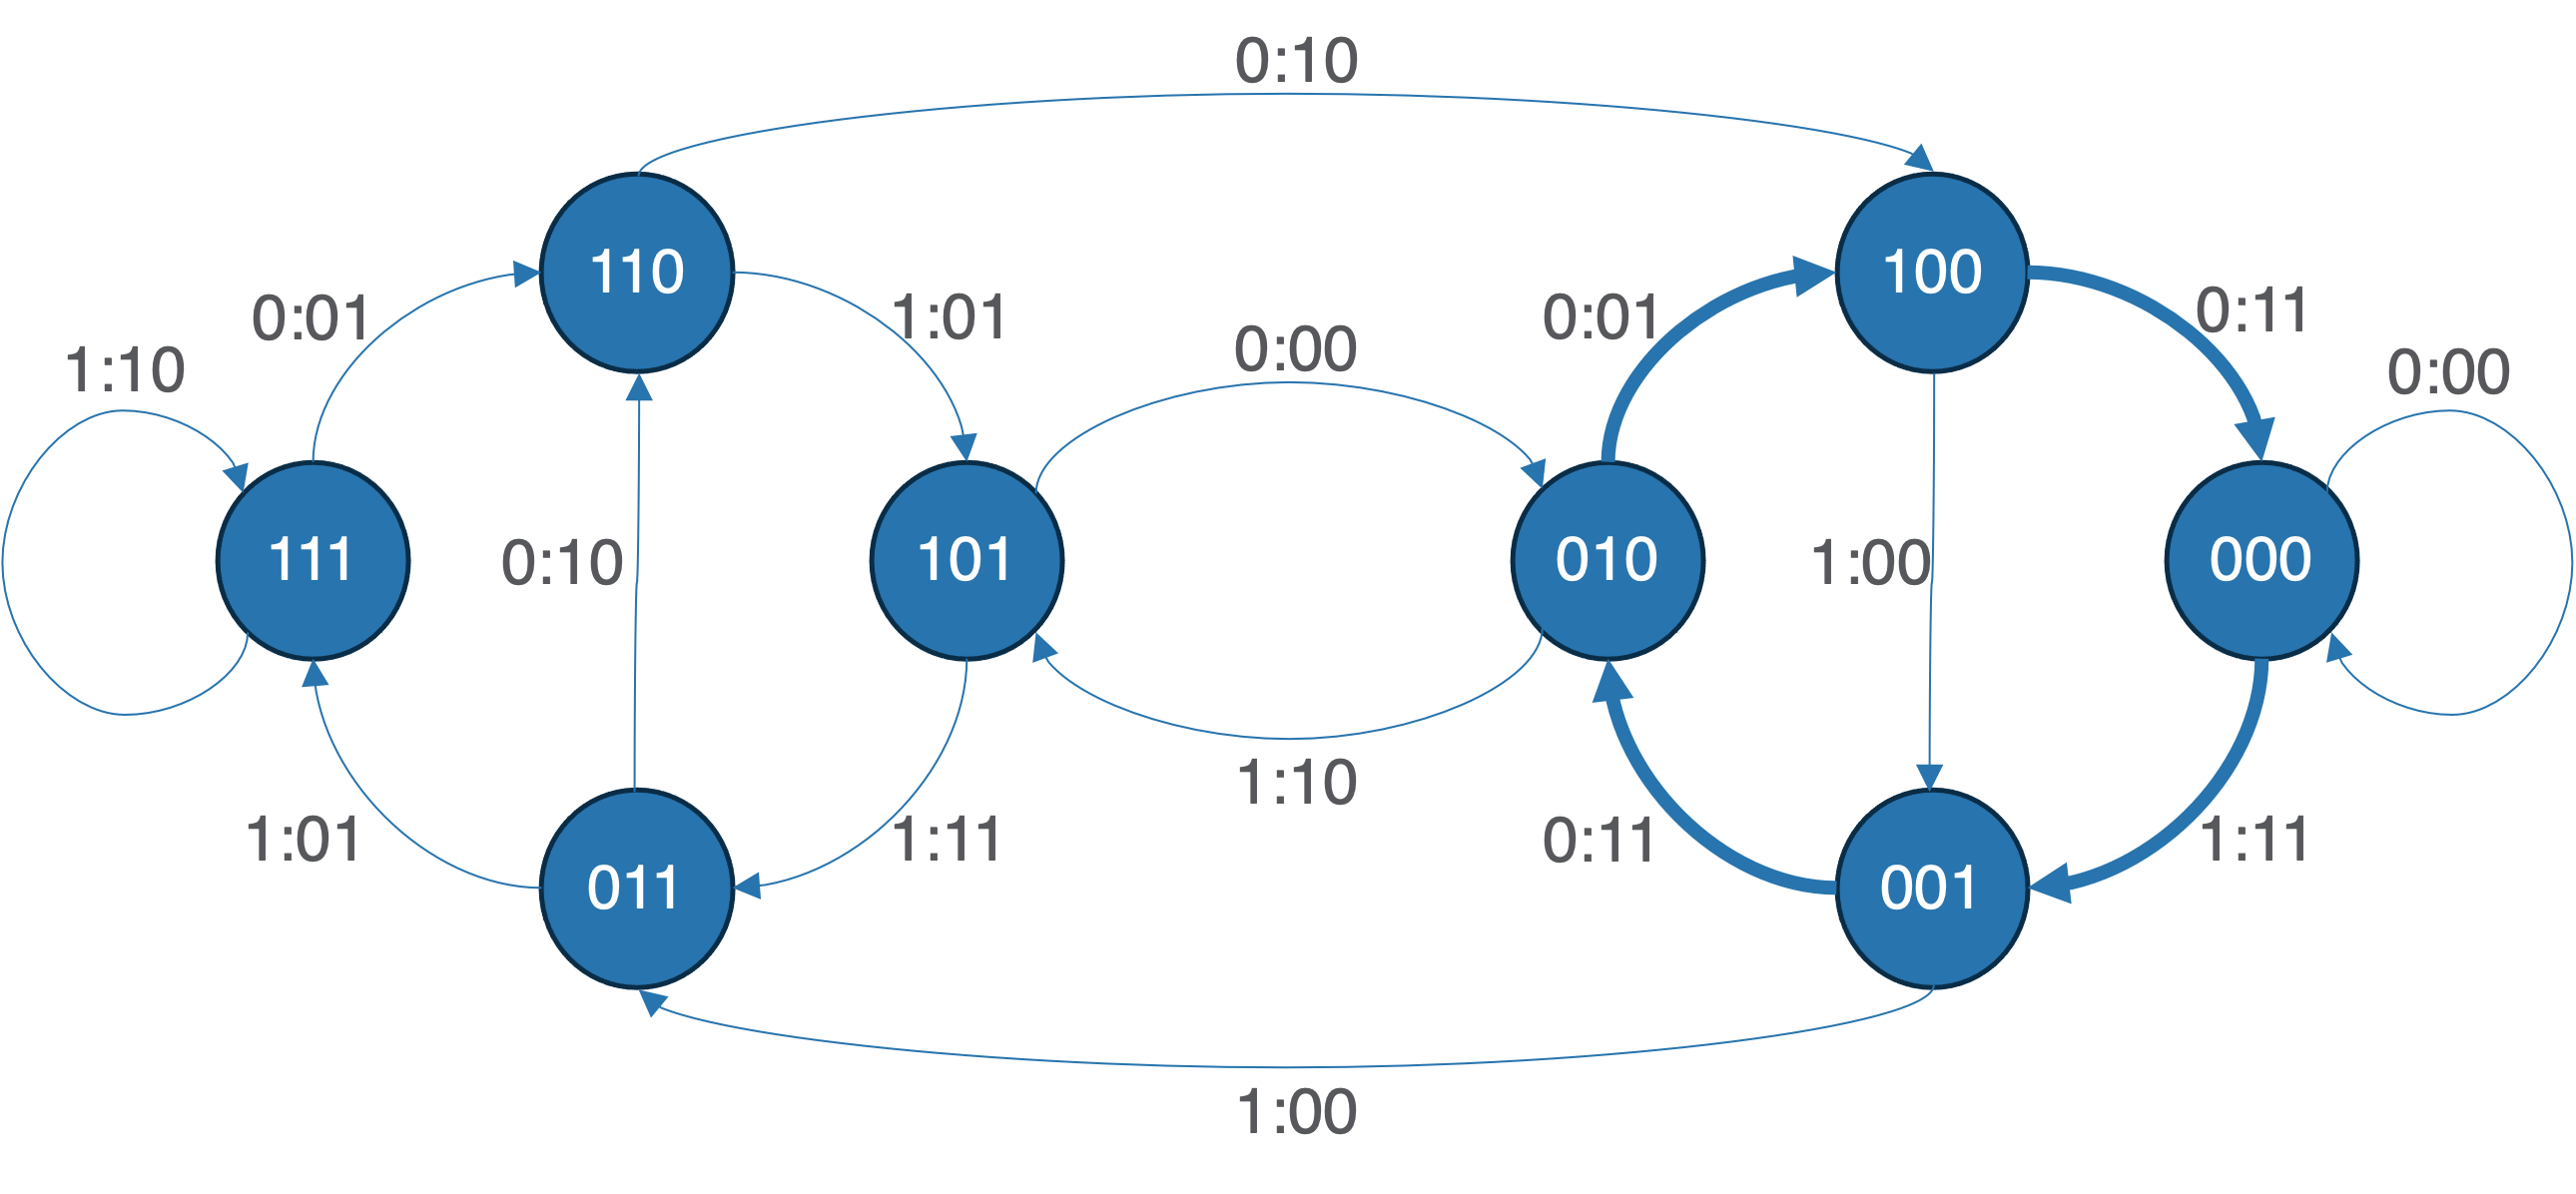
\includegraphics[height=15em]
{Figures/convolutional_code_state_diagram.png}
\caption[State diagram interpretation of a convolutional code]
{State diagram interpretation of a convolutional code}
\label{Figure:Background:ConvolutionalCodeStateDiagram}
\end{figure}
%%%%%%%%%%%%%%%%%%%%%%%%%%%%%%%%%%%%%%%%%%%%%%%%%%%%%%%%%%%%%%%%%

Each state in this diagram represents the previous $N$ message bits, i.e every possibility the values stored in the $N$ memory elements can take. Each state transition then represents updating the cascaded memory elements after a new message bit has been encoded. In this paper we will use the convention where the MSB of the state is the oldest encoded message bit. 

With this formulation, each directed edge of the state diagram $(s, s')$ is a transition with a corresponding bit-encoding pair $(u, c = (c_1, \ldots, c_k))$ such that $s' = (s_2, \ldots, s_N, u)$ and $c(D)=u(D)G(D)$ where $u(D)$ is the polynomial of the sequence $(u, s_1, s_2, \ldots, s_N)$ **. 

Putting everything together, given a starting state and a sequence of message bits $u = (u_1, \ldots, u_T)$, there exists a unique sequence of directed edges (a graph walk) on the state diagram and the sequence of corresponding bit-encoding pairs give the encoding $c$ of $u$. Shown above is an example of a state diagram where each edge is labeled by its bit-encoding pair.

\subsection{Trellis Diagram Representation}

A trellis representation (\Figure~\fref{Figure:Background:ConvolutionalCodeTrellisDiagram}) is identical in nature to the state diagram, except now each state has a unique node for different time points. Mathematically, each directed edge of the trellis $(s, s')$ for $s, s' \in S = (s^t_1, \ldots, s^t_N) | s^t_i \in \{0,1\} \text{  and  } 0 \leq t \leq T$. All other statements of ** still apply, and thus we see a walk (now a path) in the trellis graph again corresponds to a unique message $u$ and encoding $c$.

One important thing to note is that the structure of every $N$ state trellis is the same, and for two $N$ state convolution encodes, the only differences lie in the bit-encoding pair given by $G(D)$. 

%%%%%%%%%%%%%%%%%%%%%%%%%%%%%%%%%%%%%%%%%%%%%%%%%%%%%%%%%%%%%%%%%
% FIGURE: BACKGROUND: Convolutional Encoder Trellis Diagram
\begin{figure}
\centering\CaptionFontSize
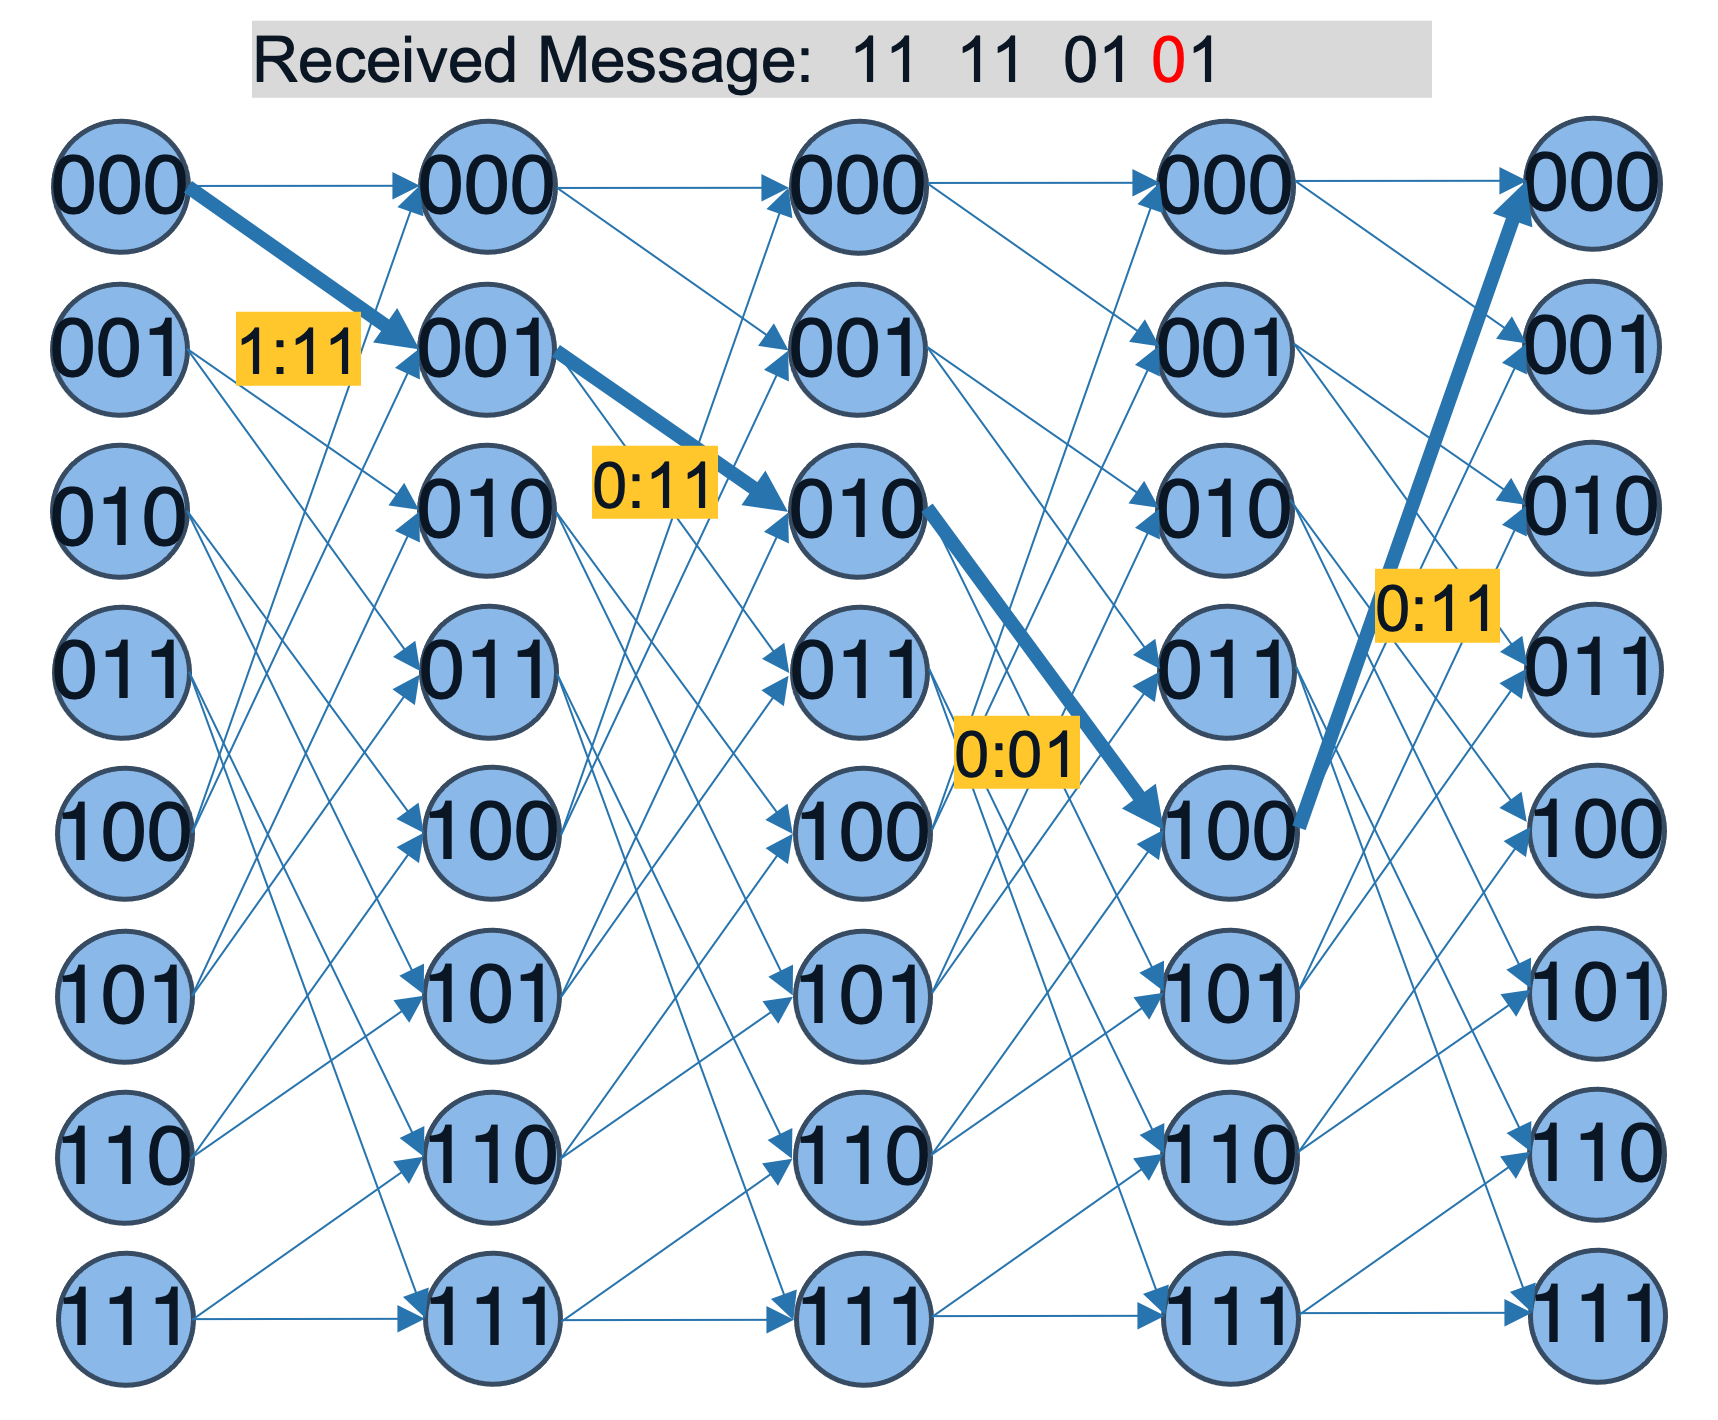
\includegraphics[height=20em]
{Figures/convolutional_code_trellis.png}
\caption[Trellis diagram interpretation of a convolutional code]
{Trellis diagram interpretation of a convolutional code}
\label{Figure:Background:ConvolutionalCodeTrellisDiagram}
\end{figure}
%%%%%%%%%%%%%%%%%%%%%%%%%%%%%%%%%%%%%%%%%%%%%%%%%%%%%%%%%%%%%%%%%

Henceforth we will denote space between the $i$th and $i+1$th column of the trellis as time points $t=i$. This is because each edge between columns represents the bit-encoding pairs, so if we split the encoded message into $T$ sections of length $k$ we can examine bit $t$ and its encodings in the trellis at time point $t$. 

\section{CRC \& Tail Biting Conditions}

Beyond the codes of interest being convolutional, we are particularly interested in CRC-aided Tail-Biting Convolutional Codes (TBCC). CRC and Tail-Biting conditions are both modifications to messages sent before encoding that streamline the transmission process. In this section we explain these modifications and the motivations behind using them.

Explanation
Cyclic Redundancy Check (CRC) is an additional form of protecting a transmitted message that appends a message with a string of bits that provides verification for the receiver that the message was received and decoded correctly. Typically, a system that includes a CRC aspect will have an agreed upon system of sending the transmitter a signal that acknowledges a successful transmission (ACK) and a signal for a failure (NACK); these are called Automatic Repeat Requests (ARQ). We call a code that has a CRC included in its encoding and decoding scheme a CRC-aided code. 

Another condition that we place on our convolutional codes is a tail biting (TB) condition. Typically, it is impractical to transmit one long continuous transmit message because it introduces complications in decoding. Instead messages are often split up and sent to the receiver in frames. In order for the decoder to decode a set of frames successfully, there must be a convention in place for the decoder to synchronize the decoding to start at the beginning of the frame. 

%%%%%%%%%%%%%%%%%%%%%%%%%%%%%%%%%%%%%%%%%%%%%%%%%%%%%%%%%%%%%%%%%
% FIGURE: BACKGROUND: CC Conditions
\begin{figure}
\centering\CaptionFontSize
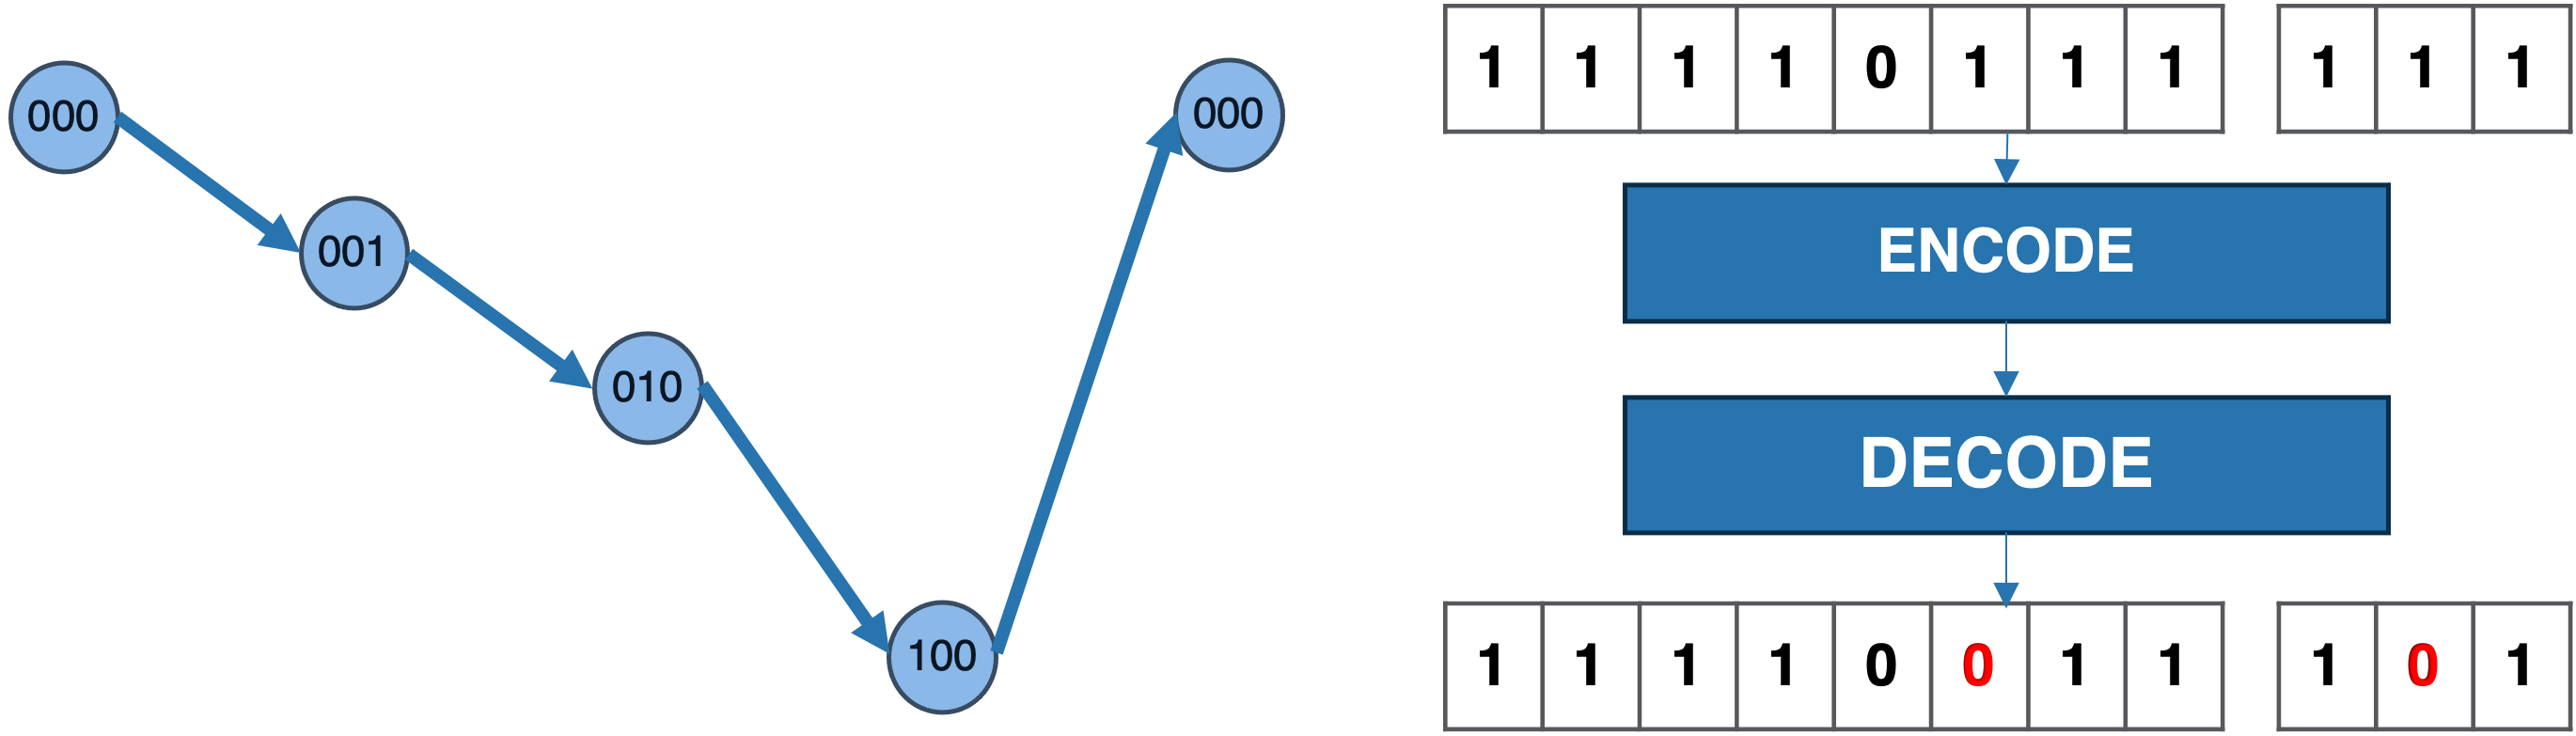
\includegraphics[width=\textwidth]
{Figures/code_conditions.png}
\caption[Visualization of CRC and Tail Biting Conditions]
{Visualization of CRC and Tail Biting Conditions. On the left is a picture of what a path in the trellis looks like when it passes the tail biting condition. On the right is an overview of how CRC is used to protect messages; the CRC portion is used to further provide error detection and correction in the original message.}
\label{Figure:Background:ConvolutionalCodeConditions}
\end{figure}
%%%%%%%%%%%%%%%%%%%%%%%%%%%%%%%%%%%%%%%%%%%%%%%%%%%%%%%%%%%%%%%%%
\TODO{fix image}
The tail biting condition is a method of frame synchronization where every frame of a sent message starts and terminates at the same state in encoding. Upon successful decoding and identification of a single frame, it then becomes easy for the decoder to identify all proceeding frames because frame length is predetermined. See \cite{Tailbiting} for more details.

\TODO{correct citing}

\section{Parallel List Viterbi Decoding (PLVD)}

Viterbi Decoding is a maximum likelihood (ML) approach to decoding a convolutional code using the Viterbi Algorithm (VA) to find the lowest metric path in the trellis with respect to the received message. We measure distance between to bit sequences with respect to a chosen metric; in this paper we choose something similar to the L2 norm, i.e the Euclidean distance between the two sequences.

As detailed in \cite{plvd}, both Serial List Viterbi Decoding (SLVD) and Parallel List Viterbi Decoding provide (PLVD) provide improved performance compared to VA, however we establish in the next section that PLVD has many algorithmic advantages that lend itself to hardware acceleration. 

\TODO{add citation}

The PLVD algorithm conventionally goes as follows. We iterate through time points starting at $t=0$. For each time point $t$, states will store a list of the $L$ paths of length $t$ with the lowest metric that end at that state $s$. For a path to have these properties, it is necessary that the path pass through the incoming edges of $s$ and thereby pass through the two states, at $t-1$ that share an edge with the $s$. WLOG let those states be $s^{t-1}_1$ and $s^{t-1}_2$ and let their respective stored lists be $l_1$ and $l_2$. To create the list of $L$ best paths at state $s$ we simply need to choose the $L$ paths with the best metric from $l_1 \cup l_2$ while taking into consideration the metric added along the incoming edges.

Formally we execute the following:

\begin{enumerate}
\item Since $t=0$ has no incoming edges, initialize and store a path starting at each state of length $0$ and with some initial metric (typically $0$).
\item For $1 \leq t \leq T$ do the following 
\begin{enumerate}
    \item For each state $s^t_i$, Let $e_1=(s^{t-1}_1, s^t_i)$ and $e_2=(s^{t-1}_2)$ be the incident edges on $s^t_i$ and $l_1$ and $l_2$ be the list of paths for $s^{t-1}_1$ and $s^{t-1}_2$.
    \item For $c$ being the received message from $t-1$ to $t$, choose the $L$ best paths from the set $\{l_1 + dist(e_1, c)\} \cup \{l_2 + dist(e_2, c)\}$ where the addition signifies adding the associated distance metric to all paths in $l_i$. 
    \item Store the chosen $L$ paths for each state.
\end{enumerate}
\item At $t = T$, we have a list of the $L$ lowest metric paths of length $T$. Out of all of these paths, choose the path with the lowest metric as our ML decoding of the received codeword.

\end{enumerate}

\subsection{Effect of TB and CRC}

In terms of execution of PLVD, the only thing that considerations for tail biting and CRC-aided codes change is our chosen path at the final $t=T$ state. Now, instead of simply choosing a path with the best metric, we must choose the path with the best metric that is tail biting and passes the CRC check. It is important to note that passing being tail biting and passing CRC are both strong conditions that drastically filter the list of valid paths at the final state. 



